\documentclass[10pt,landscape]{article}
\usepackage{multicol}
\usepackage{calc}
\usepackage{ifthen}
\usepackage[landscape]{geometry}
\usepackage{graphicx}
\usepackage{amsmath, amssymb, amsthm}
\usepackage{latexsym, marvosym}
\usepackage{pifont}
\usepackage{lscape}
\usepackage{graphicx}
\usepackage{array}
\usepackage{booktabs}
\usepackage[bottom]{footmisc}
\usepackage{tikz}
\usetikzlibrary{shapes}
\usepackage{pdfpages}
\usepackage{wrapfig}
\usepackage{enumitem}
\setlist[description]{leftmargin=0pt}
\usepackage{xfrac}
\usepackage{esvect}
\usepackage{amsmath,amsfonts,amssymb}
\usepackage[pdftex,
            pdfauthor={Javier Ferrando},
            pdftitle={Probability Cheatsheet},
            pdfsubject={A cheatsheet pdf and reference guide originally made for Stat 110, Harvard's Introduction to Probability course. Formulas and equations for your statistics class.},
            pdfkeywords={probability} {statistics} {cheatsheet} {pdf} {cheat} {sheet} {formulas} {equations}
            ]{hyperref}
\usepackage[
            open,
            openlevel=2
            ]{bookmark}
\usepackage{relsize}
\usepackage{rotating}

\usepackage{caption}
\usepackage{subcaption}
\usepackage{float}%Figures correct position
%\usepackage[font={scriptsize,it}]{caption}



 \newcommand\independent{\protect\mathpalette{\protect\independenT}{\perp}}
    \def\independenT#1#2{\mathrel{\setbox0\hbox{$#1#2$}%
    \copy0\kern-\wd0\mkern4mu\box0}} 
            
\newcommand{\noin}{\noindent}    
\newcommand{\logit}{\textrm{logit}} 
\newcommand{\var}{\textrm{Var}}
\newcommand{\cov}{\textrm{Cov}} 
\newcommand{\corr}{\textrm{Corr}} 
\newcommand{\N}{\mathcal{N}}
\newcommand{\Bern}{\textrm{Bern}}
\newcommand{\Bin}{\textrm{Bin}}
\newcommand{\Beta}{\textrm{Beta}}
\newcommand{\Gam}{\textrm{Gamma}}
\newcommand{\Expo}{\textrm{Expo}}
\newcommand{\Pois}{\textrm{Pois}}
\newcommand{\Unif}{\textrm{Unif}}
\newcommand{\Geom}{\textrm{Geom}}
\newcommand{\NBin}{\textrm{NBin}}
\newcommand{\Hypergeometric}{\textrm{HGeom}}
\newcommand{\HGeom}{\textrm{HGeom}}
\newcommand{\Mult}{\textrm{Mult}}

\geometry{top=.4in,left=.2in,right=.2in,bottom=.4in}

\pagestyle{empty}
\makeatletter
\renewcommand{\section}{\@startsection{section}{1}{0mm}%
                                {-3ex plus -.5ex minus -.2ex}%
                                {0.5ex plus .2ex}%x
                                {\normalfont\large\bfseries}}
\renewcommand{\subsection}{\@startsection{subsection}{2}{0mm}%
                                {-2ex plus -.5ex minus -.2ex}%
                                {0.5ex plus 1ex}%
                                {\normalfont\normalsize\bfseries}}
\renewcommand{\subsubsection}{\@startsection{subsubsection}{1.5}{5mm}%
                                {-2ex plus -.5ex minus -.2ex}%
                                {1ex plus 1ex}%
                                {\normalfont\small\bfseries}}
\makeatother

\setcounter{secnumdepth}{0}

\setlength{\parindent}{0pt}
\setlength{\parskip}{0pt plus 0.5ex}

% -----------------------------------------------------------------------

\usepackage{titlesec}

\titleformat{\section}
{\color{black}\normalfont\large\bfseries}
{\color{black}\thesection}{1em}{}

\titleformat{\subsection}
{\color{black}\normalfont\normalsize\bfseries}
{\color{black}\thesection}{1em}{}

\titleformat{\subsubsection}
{\color{black}\normalfont\small\bfseries}
{\color{black}\thesection}{0.5em}{}
% Comment out the above 5 lines for black and white

\begin{document}

\raggedright
\footnotesize
\begin{multicols*}{3}

% multicol parameters
% These lengths are set only within the two main columns
%\setlength{\columnseprule}{0.25pt}
\setlength{\premulticols}{1pt}
\setlength{\postmulticols}{1pt}
\setlength{\multicolsep}{1pt}
\setlength{\columnsep}{2pt}

%%%%%%%%%%%%%%%%%%%%%%%%%%%%%%%%%%%%
%%% TITLE
%%%%%%%%%%%%%%%%%%%%%%%%%%%%%%%%%%%%

\begin{center}
    {\color{black} \Large{\textbf{Multivariate Analysis}}} \\
\end{center}

%%%%%%%%%%%%%%%%%%%%%%%%%%%%%%%%%%%%
%%% ATTRIBUTIONS
%%%%%%%%%%%%%%%%%%%%%%%%%%%%%%%%%%%%
\begin{center}
\normalsize{Javier Ferrando Monsonis}
\end{center}

%\begin{center}
%    Last Updated \today
%\end{center}

% Cheatsheet format from
% http://www.stdout.org/$\sim$winston/latex/

%%%%%%%%%%%%%%%%%%%%%%%%%%%%%%%%%%%%
%%% BEGIN CHEATSHEET
%%%%%%%%%%%%%%%%%%%%%%%%%%%%%%%%%%%%


\section{PCA}\smallskip \hrule height 2pt \smallskip

    \subsection{PCA Analysis in $R^{p}$} 
    
        \begin{minipage}{\linewidth}
            \centering
            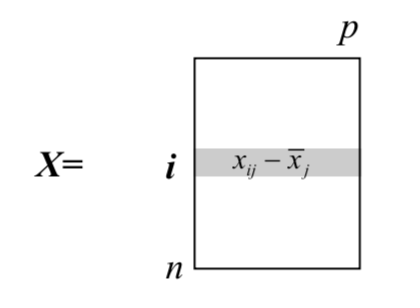
\includegraphics[width=1.5in]{X_matrix.png}
        \end{minipage}

We consider $\mathbf{X}$ as the centered dataset matrix of n observations and p features.
\break
%\vspace{5mm}
\begin{minipage}{\linewidth}
            \centering
            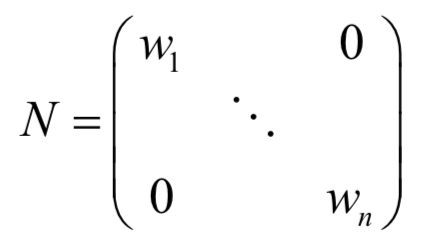
\includegraphics[width=1.1in]{N_matrix.png}
        \end{minipage}
\break
$\mathbf{N}$ is a diagonal matrix containing weights (importance) for each of the observations in the data.

$\mathbf{u}_1 \in R^{p}$ is considered a unitary vector defining a direction in $R^{p}$.

$\Psi_{1 i}$ represents the projection of the observation $i$ on $\mathbf{u}_1$. When projecting all the individuals on $\mathbf{u}_1$, we get

\begin{align*}
    \Psi_1 = \mathbf{X} \cdot \mathbf{u}_1 \\
    \end{align*}

The goal is to obtain orthogonal vectors $\mathbf{u}$ in the directions which maximizes the variance (or inertia  $I_n$) of their $\Psi$, maximizing the sum of the individual's projections on $\mathbf{u}$. So, in the case of the First Principal Component the objective function we will try to maximize is

\begin{align*}
    \max_{\mathbf{u}_1} I_{total} = \max_{\mathbf{u}_1} \displaystyle\sum_{i=1}^{n} w_i \Psi_{1 i}^2 = \Psi_{1}^\intercal \mathbf{N} \Psi_{1} = \mathbf{u}_1^\intercal \mathbf{X}^\intercal \mathbf{N}  \mathbf{X} \mathbf{u}_1 \\
    \end{align*}
Subject to $\mathbf{u}_1 \mathbf{u}_1^\intercal = \lVert \mathbf{u}_1  \rVert ^2_2 = 1$
\newline

Method of Lagrange multipliers $\to$ $\mathcal {L}(x,y,\lambda )=f(x,y)-\lambda g(x,y),$

\begin{align*}
    \ell = \mathbf{u}_1^\intercal \mathbf{X}^\intercal \mathbf{N} \mathbf{X} \mathbf{u}_1 - \lambda_1(\mathbf{u}_1^\intercal \mathbf{u}_1 - 1)
    \end{align*}


Setting $\frac{\partial \ell}{\partial u} = 0$

\begin{align*}
    2 \mathbf{X}^\intercal \mathbf{N} \mathbf{X} \mathbf{u}_1 - 2 \lambda_1 \mathbf{u}_1 = 0
    \end{align*}
\begin{align*}
    \mathbf{X}^\intercal \mathbf{N} \mathbf{X} \mathbf{u}_1  = \lambda_1 \mathbf{u}_1
    \end{align*}

Since we are using a centered matrix, $\mathbf{X}^\intercal \mathbf{N} \mathbf{X} = Cov(\mathbf{X})$, $\mathbf{u}_1$ represents an eigenvector of $Cov(\mathbf{X})$ and $\lambda_1$ its associated eigenvalue. Taking the largest $\lambda_1$ will give the eigenvector with maximum variance (First Principal Component).
%Cov(\mathbf{X}

$\Psi_{\alpha} \in R^n$ where each component represent the projection of each individual $i$ on the Principal Component $u_{\alpha}$.

Since $u_{1}$ is a unitary vector we deduce from previous formulas that  $\Psi_{1}^\intercal \mathbf{N} \Psi_{1} = \lambda_{1} = var(\Psi_1)$

\begin{align*}
I_{total}= \sum_{j=1}^{p} \sum_{i=1}^{n} w_i (x_{ij} - \overline{x}_j)^2 = \sum_{j=1}^{p} var(x_j) = \sum_{\alpha=1}^{p} \lambda_{\alpha}
\end{align*}

Projected inertia on the first axis
\begin{align*}
I_{1}= \sum_{i=1}^{n}\frac{1}{n}\Psi_{1 i}^2 = \lambda_1
\end{align*}

When working with  standardized $\mathbf{X}$ matrix, $\mathbf{X}^\intercal \mathbf{N} \mathbf{X} = Cor(\mathbf{X})$

\subsection{PCA Analysis in $R^{n}$}
$\mathbf{v}_1 \in R^{n}$ is considered a unitary vector defining a direction in $R^{n}$. $\varphi_{1j}$ denotes the projections of variable j onto $\mathbf{v}_1$, $\mathbf{X}^\intercal \mathbf{N}^{1/2} \mathbf{v}_1$, when using a standardized matrix, $\varphi_{1} = cor(\mathbf{X}, \Psi_{1})$. The function to maximize is

\begin{align*}
    \max_{\mathbf{v}_1} I_{total} = \max_{\mathbf{v}_1} \displaystyle\sum_{j=1}^{p} \varphi_{1j}^2 = \varphi_{1}^\intercal \varphi_{1} = \mathbf{v}_1^\intercal \mathbf{N}^{1/2} \mathbf{X} \mathbf{X}^\intercal \mathbf{N}^{1/2} \mathbf{v}_1 \\
    \end{align*}

Subject to $\mathbf{v}_1 \mathbf{v}_1^\intercal = \lVert \mathbf{v}_1  \rVert ^2_2 = 1$

Following the same optimization procedure that in $R^{p}$ we get

\begin{align*}
    \mathbf{N}^{1/2} \mathbf{X} \mathbf{X}^\intercal \mathbf{N}^{1/2} \mathbf{v}_1 = \lambda_{1} \mathbf{v}_1 \\
    \end{align*}
    
Transition relationships between both fits
\begin{align*}
    \mathbf{u}_{\alpha} = \lambda^{-1/2} \mathbf{X}^\intercal \mathbf{N}^{1/2} \mathbf{v}_\alpha
    \end{align*}

\begin{align*}
    \mathbf{v}_{\alpha} = \lambda^{-1/2} \mathbf{N}^{1/2} \mathbf{X} \mathbf{u}_\alpha
    \end{align*}


\subsection{Singular Value Decomposition}

Let's call $\mathbf{M} = \mathbf{N}^{1/2} \mathbf{X}$
\begin{align*}
    \mathbf{M} \mathbf{u}_{\alpha} = \mathbf{v}_\alpha \sqrt{\lambda_{\alpha}}
    \end{align*}
    
\begin{align*}
\mathbf{M}^\intercal \mathbf{v}_\alpha =  \mathbf{u}_{\alpha} \sqrt{\lambda_{\alpha}}
    \end{align*}
In matrix form
\begin{align*}
\mathbf{M} \mathbf{U} = \mathbf{V} \Lambda^{1/2} \to \mathbf{M} = \mathbf{V} \Lambda^{1/2} \mathbf{U}^\intercal
    \end{align*}
    
So, the singular values of $\mathbf{M}$ are the ones contained in the diagonal of $\Lambda^{1/2}$, been the eigenvalues of $\mathbf{M} \mathbf{M}^\intercal = \mathbf{N}^{1/2} \mathbf{X} \mathbf{X}^\intercal \mathbf{N}^{1/2}$ the square of  the singular values obtained.

\subsection{Attributes from PCA RFactominer}
Having pca\$ind and pca\$var as the objects returned by PCA function.

\begin{itemize}
    \item coord
    
    Values of the projections of individuals and variables on the Principal Components

    \item cos2
    
     Contribution (importance) of a component to the squared distance of the observation to the origin (G) in the original cloud of points. Quality of the representations.
    
\begin{align*}
    cos^2(i,\alpha) = \frac{\Psi_{\alpha i}^2}{d_{i,G}^2}
    \end{align*}
\begin{align*}
    cos^2(j,\alpha) = \frac{\varphi_{\alpha j}^2}{s_{j}^2}
    \end{align*}
    
    \item contrib
    
    Contribution of an individual or variable to the variance explained by a component $\alpha$

\begin{align*}
    ctr(i,\alpha) = \frac{w_{i}\Psi_{\alpha i}^2}{\lambda_{\alpha}}
    \end{align*}
\begin{align*}
    ctr(j,\alpha) = \frac{\varphi_{\alpha j}^2}{\lambda_{\alpha}}
    \end{align*}
    
    Factominer \$contrib multiplies by 100 these values, so the sum of contributions is 100.
    
    \item dist(\$ind)
    
    \item cor(\$var)
    
    Correlation between a component and a variable $\varphi_{\alpha j} = cor(x_{j}, \Psi_{1})$ (standardized $\mathbf{X}$). How much information they share.
\end{itemize}    
\subsection{Supplementary variables}
\subsubsection{Categorical variables}
In $R^p$, its displayed the projection of the centroid of the individuals which share each of the categories onto the Principal Components.

\subsubsection{Continuous variables}
In $R^n$, the correlation between the supplementary variable and the Principal Components are shown.

\newpage

\section{Correspondence Analysis}\smallskip \hrule height 2pt

\subsection{CA}

\begin{minipage}{3.15in}
    \centering
            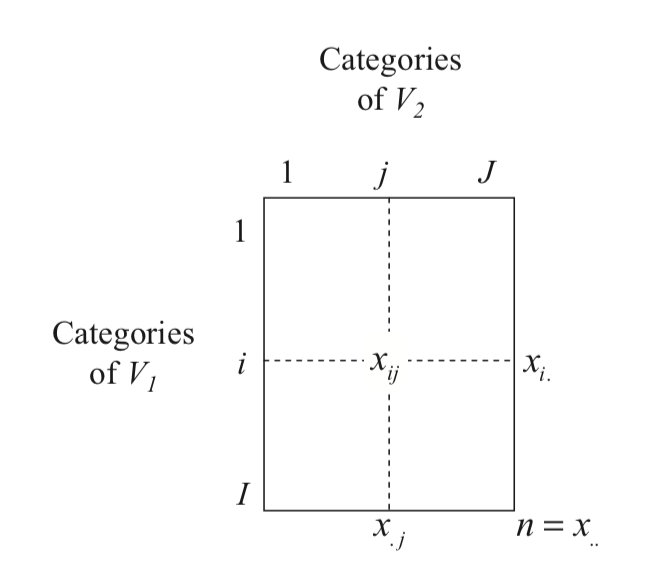
\includegraphics[width=1.6in]{contingency_table.png}
        \end{minipage}
\break

\begin{align*}
    x_{i\bullet} = \sum_{j=1}^{J} x_{ij} \quad  x_{\bullet j} = \sum_{i=1}^{I} x_{ij} \quad n = x_{\bullet\bullet} = \sum_{i,j} x_{ij}
    \end{align*}
    
In CA it is also considered the probability tables associated with contingency tables as the general term $f_{ij} = x_{ij} /n$, the probability of carrying both the categories i (of V1) and those of j (V2)

\begin{align*}
    f_{i\bullet} = \sum_{j=1}^{J} f_{ij} \quad  f_{\bullet j} = \sum_{i=1}^{I} f_{ij} \quad f_{\bullet\bullet} = \sum_{i,j} f_{ij} = 1
    \end{align*}

\subsubsection{Independence Model and $\chi^2$ Test}

\begin{minipage}{\linewidth}
    \centering
            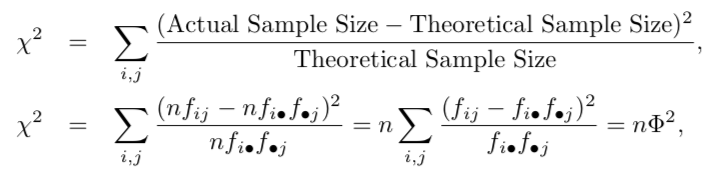
\includegraphics[width=3in]{chi_square_ca.png}
        \end{minipage}


If each category of $V_1$ where independent from every category of $V_2$

\begin{align*}
    \forall i,j \quad \frac{f_{ij}}{f_{i \bullet}} = f_{\bullet j}
    \end{align*}

$f_{\bullet j}$ is the conditional probability $P(j|i) = \frac{P(j,i)}{P(i)}$. So, the probability of carrying category $j$ when carrying category $i$ does not depend on the category $i$ (in the independence model).
\break

\begin{minipage}{\linewidth}
    \centering
            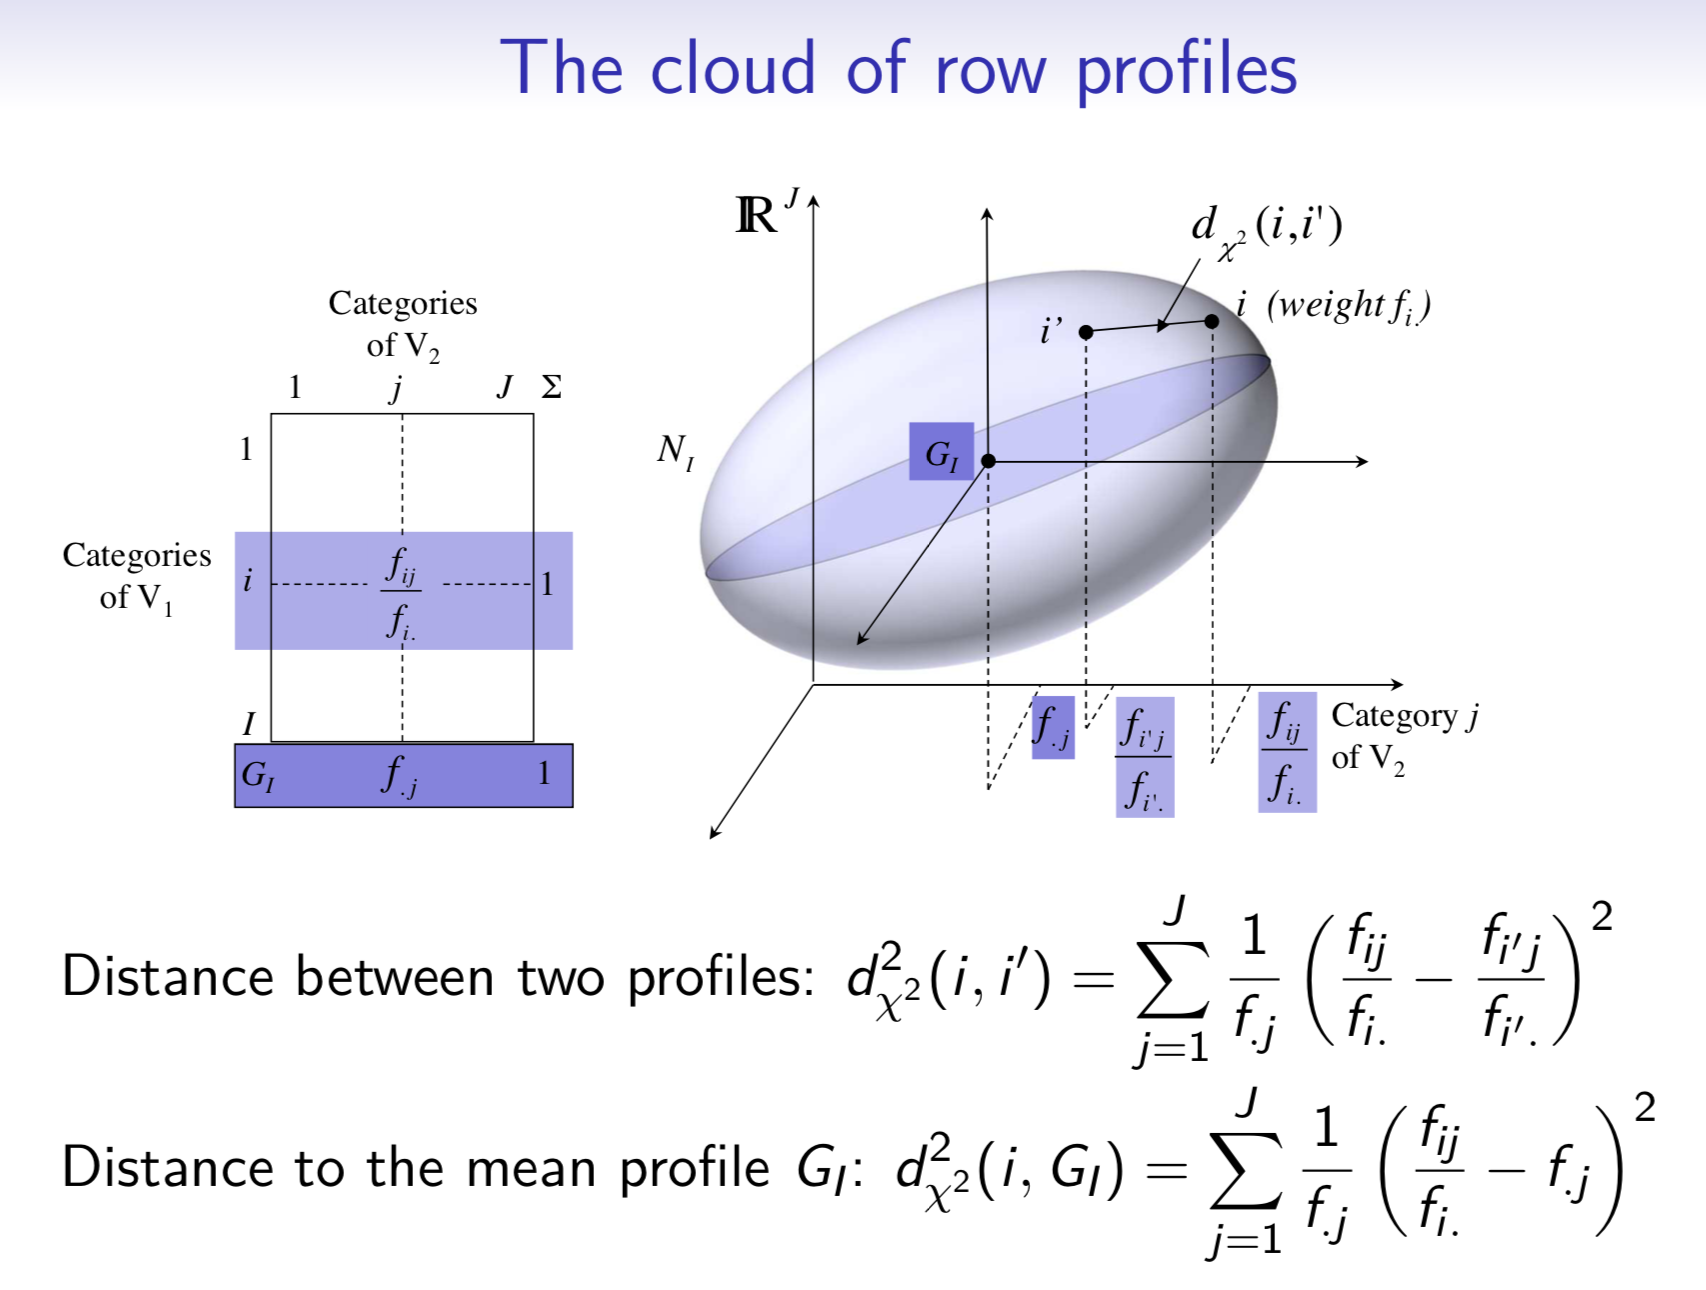
\includegraphics[width=2.8in]{cloud_of_row_profiles.png}
        \end{minipage}
        
\begin{minipage}{\linewidth}
    \centering
            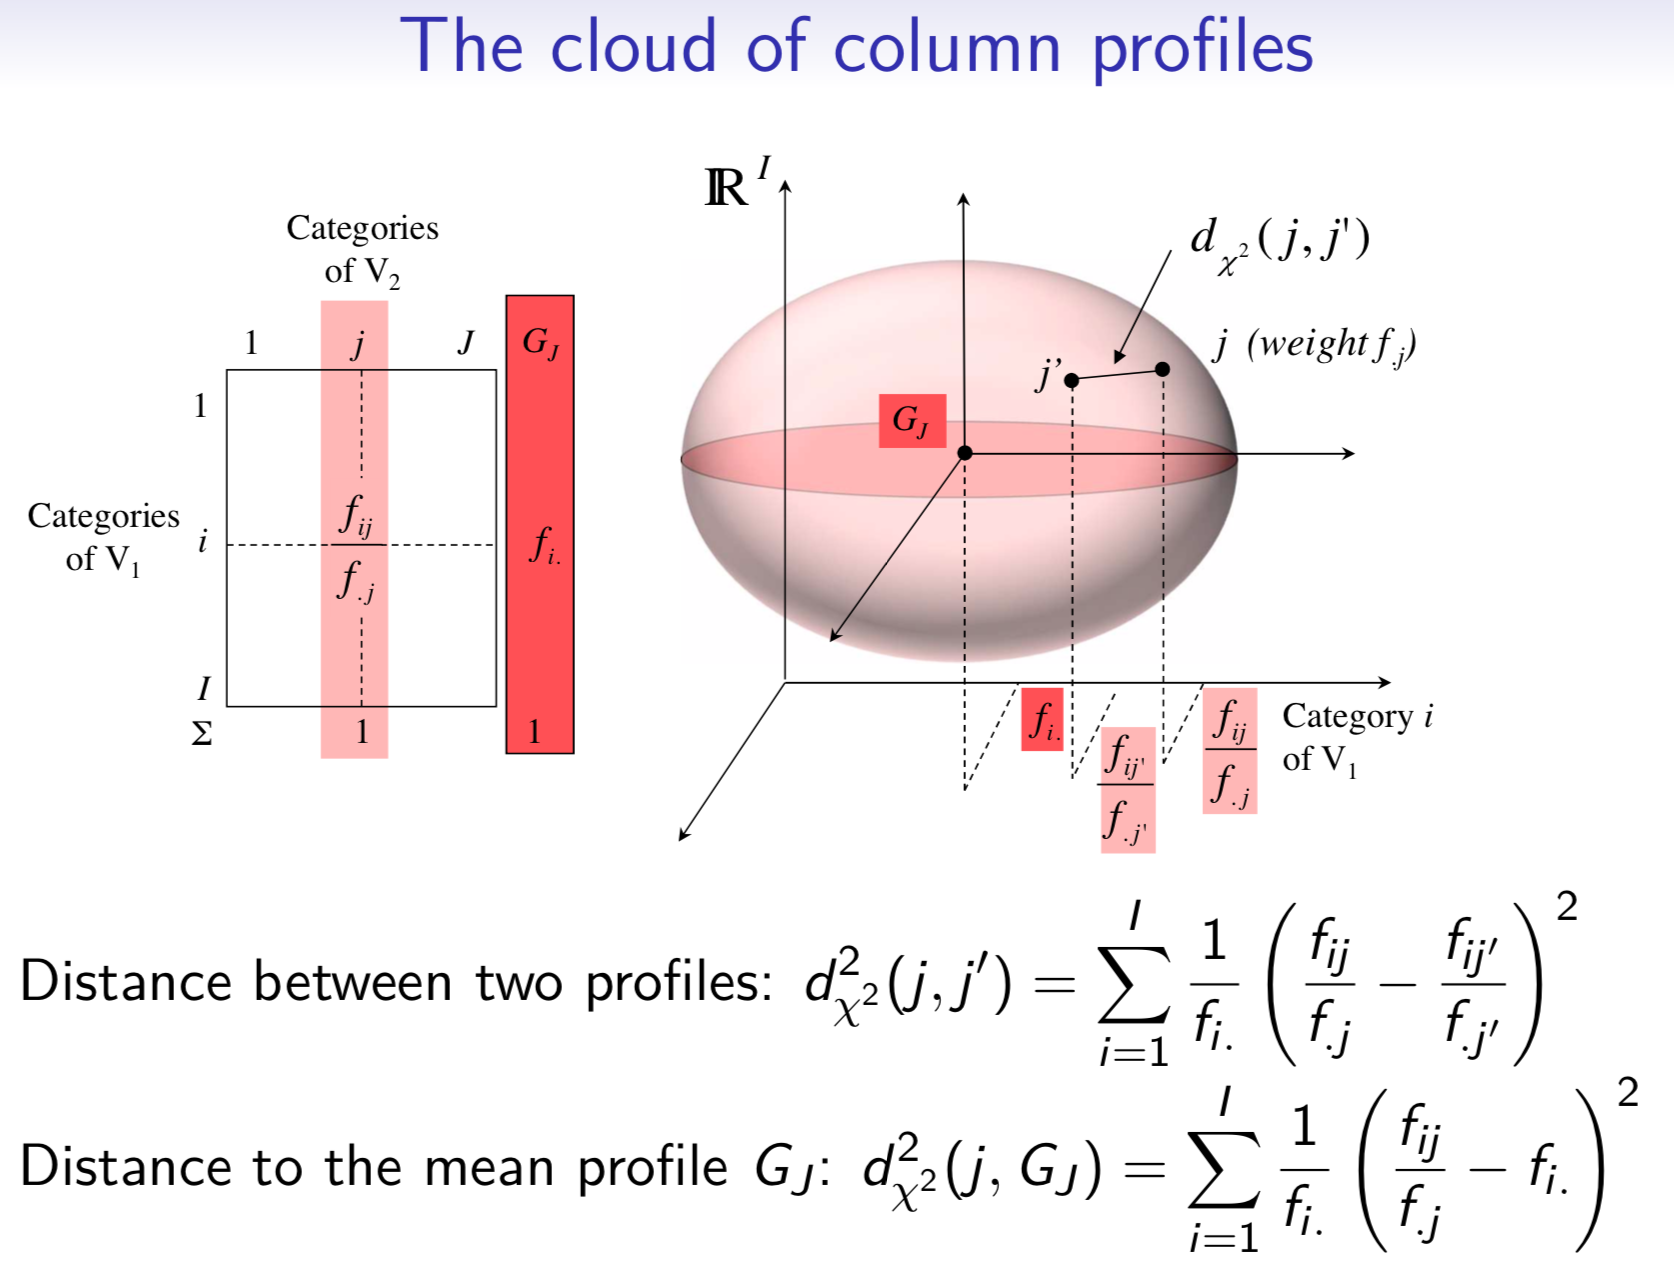
\includegraphics[width=2.8in]{cloud_of_column_profiles.png}
        \end{minipage}

The further the data is from independence, the more the profiles spread from the origin

\begin{minipage}{\linewidth}
    \centering
            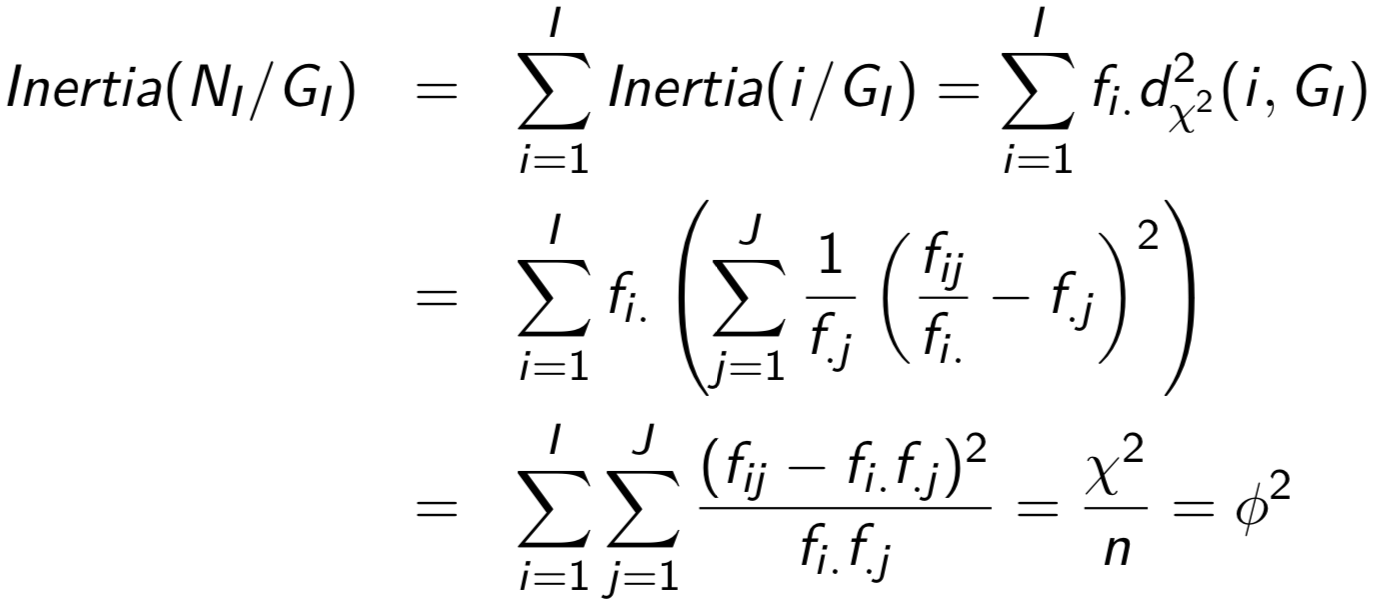
\includegraphics[width=2.5in]{inertia_ca.png}
        \end{minipage}
\break

$\phi^2$ measures the strength of the link

\begin{minipage}{\linewidth}
    \centering
            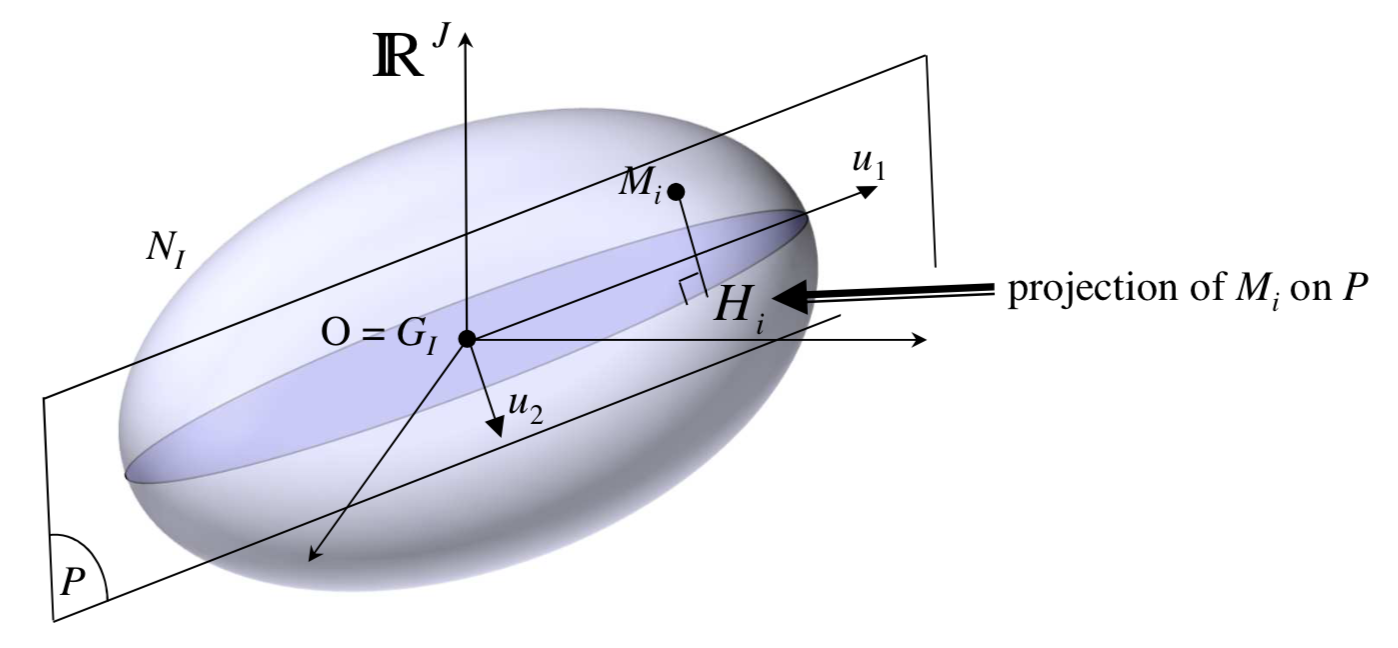
\includegraphics[width=2.5in]{plane.png}
        \end{minipage}
\break
Find \textbf{P} that maximizes $\sum_{i=1}^{I}f_{i\bullet}(OH_i)^2$


\section{Decision trees}\smallskip \hrule height 2pt \smallskip

\begin{figure}[H]
\centering
\begin{minipage}{0.5\linewidth}
  \centering
  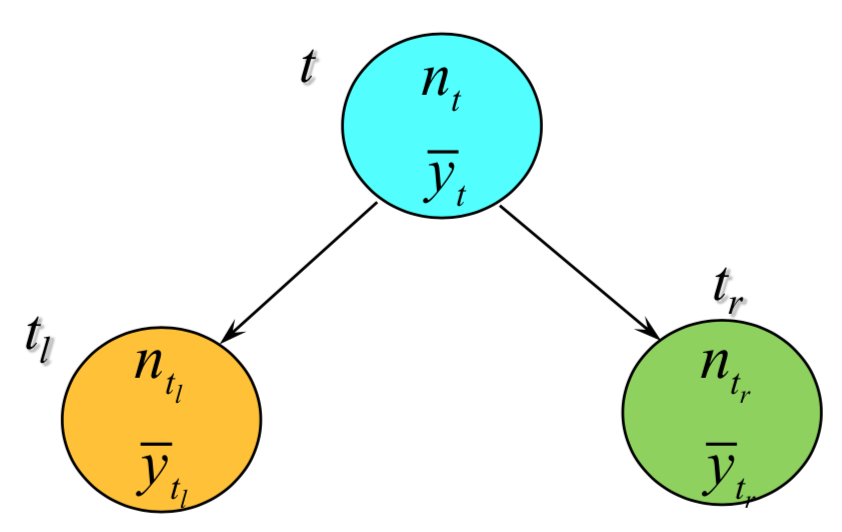
\includegraphics[width=1.32in]{regression_tree.png}
  \captionof*{figure}{\scriptsize{\textit{Regression tree}}}
  \label{fig:test1}
\end{minipage}%
\begin{minipage}{0.5\linewidth}
  \centering
  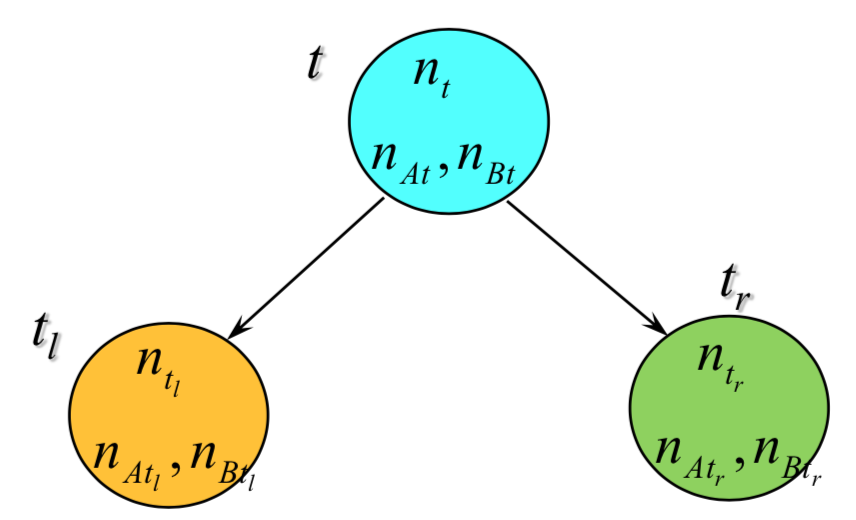
\includegraphics[width=1.4in]{classification_tree.png}
  \captionof*{figure}{\scriptsize{\textit{Classification tree}}}
  \label{fig:test2}
\end{minipage}
\end{figure}

        
\subsection{Split criterion}
\subsubsection{AID} 

AID split criterion is based on decomposition of variance
\begin{align*}
    \sum_{i=1}^{n_t} (y_i - \overline{y}_t)^2 =\sum_{k=1}^{q} n_{t_k}(\overline{y}_{t_k} - \overline{y}_t) + \sum_{k=1}^{q} \sum_{i \in t_k}^{n_{t_k}}(y_{i} - \overline{y}_{t_k})^2\\
\end{align*}

Where the first term of the equation refers to the variance between child nodes $t_k$ and parent node $t$ and the second term, the variance within child nodes.

$y_i$ denotes the response for every individual $i$ out of $n_t$ (number of individuals in node $t$), $q$ the number of children nodes (2 in a binary tree), $\overline{y}_t$ the mean response in node $t$.

We can now calculate the F statistic, $F={\frac  {{\text{between-nodes variability}}}{{\text{within-nodes variability}}}}$

\begin{align*}
    F = \frac{\sum_{k=1}^{q} n_{t_k}(\overline{y}_{t_k}  - \overline{y}_t) / q - 1 }{\sum_{k=1}^{q} \sum_{i \in t_k}^{n_{t_k}}(y_i - \overline{y}_{t_k})^2 / n - q} \\
\end{align*}

The goal is to obtain the feature and its cutpoint that leads to the highest F value, increasing as much as possible the between-nodes variability.



\subsubsection{CHAID}

CHAID split criterion is based on the Chi-square statistic comparing the frequency of each class and children node



\begin{align*}
    \chi^2 = \sum_{k=1}^{m} \sum_{j=1}^{q} \frac{\Big(n_{kt_j} - n_{k\cdot} \cdot \frac{n_{\cdot t_j}}{n_t}\Big )^2} {n_k \cdot \frac{\cdot n_{t_j}}{n_t}} \\
\end{align*}

The goal is to obtain the feature and its cutpoint that leads to the highest $\chi^2$ value.

\subsection{Impurity of a node}
$p(j|t)$ probability of class $j$ in node $t$
\subsubsection{Categorical response}

\begin{itemize}
    \item Gini
    
    \begin{align*}
    i(t) = \sum_{i \neq j} p(j|t) p(i|t) = 1 - \sum_{j}^{q} p_j^2 \\
\end{align*}

    \item Information (Entropy)
    
    \begin{align*}
    i(t) = \sum_{j} p(j|t) log_2 p(j|t) \\
\end{align*}
    
\subsubsection{Continuous response}

    \item Variance
\end{itemize}

     \begin{align*}
        i(t) = \frac{\sum_{i \in t} (y_i - \overline{y}_t)}{n} \\
    \end{align*}
    
The objective is to maximize the decrement of impurity between the parent and its children.
The decrement of impurity is defined as follows

     \begin{align*}
        \Delta i(t) = i(t) - \frac{n_{tl}}{n_t} i(t_l) - \frac{n_{tr}}{n_t}i(t_r) \\
    \end{align*}
    
\subsection{Cost of the tree}
Cost of a node (classification tree)

     \begin{align*}
        r(t) = 1-max_j p(j|t) \\
    \end{align*}
    
Cost of a node (regression tree)

    \begin{align*}
        r(t) = \frac{1}{n_t} \sum_{i \in t}^{n_t} (y_{i} - \overline{y}_t)^2 \\
    \end{align*}

Cost of a classification tree

     \begin{align*}
        R(t) = \frac{\sum_{t \in T} p(t)r(t)}{r(root)} \cdot 100 \\
    \end{align*}

Cost of a regression tree (guessing)

\begin{align*}
        R(t) = \sum_{t \in T} \frac{1}{n_t} \sum_{i \in t}^{n_t} (y_{i} - \overline{y}_t)^2 \\
    \end{align*}

The criterion to optimize is to minimize $R(t)$

\subsubsection{Penalization of complexity}
Since the previous objective function would lead to large trees, we use $\alpha$ as a complexity parameter to control its size.\newline

The new objective function becomes

\begin{align*}
        Min(R(t) + \alpha |T|) \\
    \end{align*}
    
\subsubsection{Model selection}

Training data: train trees with increasing values of $\alpha$. Each obtained tree will have $Min(R(t))$ within the set of trees with complexity $\alpha$ $(|T|)$.
\newline
Validation data: calculate every tree $R(T)$ using validation data and get the optimum one.

\subsection{ROC and Concentration curves}

\begin{minipage}{\linewidth}
    \centering
            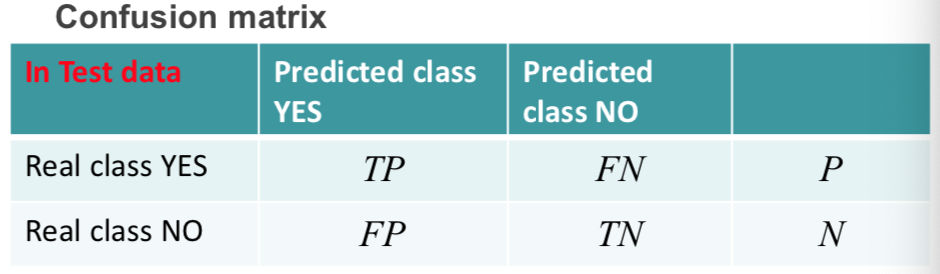
\includegraphics[width=2.5in]{conf_mat.png}
        \end{minipage}
\break

\begin{align*}
    Precision = \frac{1}{2}\bigg[ \frac{TP}{TP + FP} +  \frac{TN}{TN + FN}\bigg]\\
\end{align*}

\begin{align*}
    Accuracy = 1 - \frac{FN + FP}{n}\\
\end{align*}

\begin{align*}
    Recall = Sensitivity = \frac{TP}{P}\\
\end{align*}


    
\section{Association Rules}\smallskip \hrule height 2pt \smallskip

    \subsection{Support} 
    
\begin{align*}
    Support(I_k) = \frac{|T|\{I_k\}	\subseteq T}{|\tau|} \\
\end{align*}
    

Probability of finding $I_k$ itemset in the set $T$ of transactions

    \subsection{Confidence} 
    
\begin{align*}
    Confidence(LHS \to RHS) = \frac{Support(LHS,RHS)}{Support(LHS)} \\
\end{align*}
    

Probability of RHS, having occurred LHS 

\begin{align*}
P(RHS|LHS) = \frac{P(RHS,LHS)}{P(LHS)} \\
\end{align*}

    \subsection{Lift} 
    
\begin{align*}
    Lift(LHS \to RHS) = \frac{Support(LHS,RHS)}{Support(LHS) \cdot Support(RHS)} \\
\end{align*}
    
Lift $\in [0,\infty]$, can be interpreted as how much better is a rule than a random prediction of the consequent (RHS).For Lift values $< 1$, should rely on Support(RHS) rather than following the rule.



\end{multicols*}
\end{document}
